%
% Title:  "Template for final thesis paper (Bachelor/Master)"
% File:   "thesis.tex"
% Author: "s0nda"
%
% Inspired from the tum-thesis-latex of Florian Walch
% [https://github.com/fwalch/tum-thesis-latex]

%======================================================
% set paper format A4 and one-sided
\documentclass[paper=a4,oneside,footsepline,headinclude=false,footinclude=false,fontsize=11pt,listof=totoc,bibliography=totoc]{scrbook}

%======================================================
% import packages and configurations
%======================================================
%
% settings.tex
%
%======================================================
% import packages
%======================================================
\usepackage[utf8]{inputenc}%\usepackage[T1]{fontenc}
\usepackage[ngerman]{babel}
\usepackage[autostyle]{csquotes}% load "csquotes" when working with "babel" and "bibtex" to avoid
                                % the warning "'babel/polyglossia' detected but 'csquotes' missing".
\usepackage{amsmath,amsthm,amssymb}
%\usepackage[sc]{mathpazo}% sc = small-cap
\usepackage{mathptmx}% supports Adobe Times Roman (or equivalent) as default text font.
\usepackage{bm}% display bold maths symbols.
\usepackage{float}% used with \begin{figure}[H] to set fixed position.
\usepackage{graphicx}
\usepackage{caption}
\usepackage{colortbl,xcolor}
\usepackage{imakeidx}% create index for later looking-up
\usepackage{ifthen}% conditional statements (if then else)
\usepackage{hyperref}
\usepackage{hypcap}
\usepackage[backend=biber,style=numeric,]{biblatex}% bibliography processor [biber] for BibLatex,
                                                   % [style=alphabetic,]


%======================================================
% configurations
%======================================================
\makeindex % create index for later looking-up
\setlength\parindent{0pt}% set \noindent for entrie file
%
% define variable for language:
%   de : Deutsch
%   en : English
\newcommand{\lang}{en}% default English.
\renewcommand{\lang}{de}% (redundant). Set German as active language.
%
% change the value \proofname (italic "Proof"/"Beweis" by default)
% and its style to bold (\bfseries) and uppercase (\textup).
\addto{\captionsngerman}{%
  \def\proofname{\textbf{\textup{Beweis.}}}
}
%
% command for setting indentation and parskip in minipage.
\setlength{\parskip}{\medskipamount}% set vertical spacing between two paragraphs (glocal), \parskip = paragraph skip
\makeatletter 
\newcommand{\@minipagerestore}{%
  \setlength{\parindent}{0pt}% set indentation at paragraph begin (local)
  \setlength{\parskip}{\medskipamount}% set vertical spacing between two paragraphs (local, minipage), \parskip = paragraph skip
}
\makeatother
%
% define new theorem style
\newtheoremstyle{mytheoremstyle}% name of the style to be used
  {\topsep}% measure of space to leave above the theorem. E.g.: 3pt
  {\topsep}% measure of space to leave below the theorem. E.g.: 3pt
  {\itshape}% name of font to use in the body of the theorem
  {0pt}% measure of space to indent
  {\bfseries}% name of head font
  {. }% punctuation between head and body
  { }% space after theorem head; " " = normal interword space
  {\thmname{\textbf{#1}}\thmnumber{ #2}\thmnote{ (#3)}}
%
%\theoremstyle{mytheoremstyle}

%======================================================
% define new environments
%======================================================
\theoremstyle{mytheoremstyle}% set theorem style
\newtheorem{definition}{Definition}[section]% numbered due to [section]
\newtheorem{theorem}[definition]{Theorem}% numbered due to [defintion]
%
% define new environment for Example. First argument #1
% has default value [Example], that means, the calling
% "\begin{example} ABCD \end{example}" yields
% "Example. ABCD". The whole example-environment is
% within a \par environment (paragraph).
\newenvironment{example}[1][%
  \ifthenelse{% if
    \equal{\lang}{de}
  }{% then
    Beispiel.
  }{% else
    Example.
}]{%
  \par{{\bfseries #1}}
}{\par}
%


%======================================================
% import bibliography (bibtex)
%======================================================
\addbibresource{bibliography.bib}

%=====================================================%
%                                                     %
%             BEGIN DOCUMENT                          %
%                                                     %
%=====================================================%
\begin{document}

%======================================================
% Cover Page
%======================================================
\pagestyle{empty}% turn-off page numbering
%
% cover.tex
%
\begin{center}
  {\Huge \textsc{\textbf{Bachelorarbeit}}}\\
  \vspace*{2.cm}
  {\Large Titel der Bachelorarbeit}\linebreak\\
  {\huge \textbf{Satz von Wilson}}\\
  \vspace*{3.cm}
  {\Large Verfasserin}\linebreak\\
  {\LARGE Esra Solmaz}\\
  \vspace*{3.cm}
  {\Large angestrebter akademischer Grad}\linebreak\\
  {\LARGE Bachelor of Education (BEd.)}
\end{center}
\vspace*{2.cm}

{\Large Wien, im Monat Februar 2021}
\vspace*{2.cm}

{\Large
  {\def\arraystretch{1}\tabcolsep=10pt % space between rows = 1, space between cols = 10pt 
    \begin{tabular}{@{}ll} % @{} removes padding space left from first column
      Studienkennzahl lt. Studienblatt: & UA 198 410 420 02 \\
      \rule{0pt}{3ex}%  EXTRA vertical height 
      Studienrichtung lt. Studienblatt: & Bachelorstudium Lehramt Sek (AB) \\
                                        & Lehrverbund UF Mathematik \\
      \rule{0pt}{3ex}%  EXTRA vertical height 
      Betreuer & Herr Mag. Dr. Andreas Ulovec
    \end{tabular}
  }
}


%======================================================
%\pagenumbering{roman}% set page numbering (alph,roman,arabic).
\frontmatter{}% start page numbering in lowercase Roman style.

%======================================================
% Abstract
%======================================================
\pagestyle{plain}% turn-on page numbering
%
% abstract.tex
%
\chapter{Abstract}

%Text für Abstract.

\begin{center}
    {\itshape ``Die Zahl ist das Wesen aller Dinge.''}
    
    {\itshape ``Das Universum ist auf der Macht der Zahlen aufgebaut.''}
    
    - Pythagoras von Samos, 570-500 v.Chr., griechischer Philosoph und Mathematiker -
\end{center}

\newpage


%======================================================
% Table of Contents
%======================================================
\tableofcontents

%======================================================
\mainmatter{}% set page numbering in Arabic style.

%======================================================
% Chapter 1
%======================================================
%
% chap001.tex
%

\chapter{Primzahlen}

%======================================================
\section{Primzahlbegriff und geschichtliche Aspekte}
%======================================================
\begin{definition}[Primzahl]
``Eine Primzahl ist eine natürliche Zahl $p > 1$, die nur 
die trivialen Teiler besitzt, d.h. deren einzige Teiler
1 und sie selbst sind'' \cite{schichlsteinbauer}, S. 23.
\end{definition}
\vspace{-.5cm}

\begin{minipage}{0.65\linewidth}
Die Primzahlen sind nicht vor einer kurzen Zeit erfunden
worden. Schon vor mehrere hunderte von Jahren hatten sich
die Mathematiker mit den Primzahlen beschäftigt.
Hinsichtlich der Mathematiker, die als erste die Primzahlen
untersuchten, sind die Mathematiker der pythagoräischen
Schule (ab 500 bis 300 v. Chr.). Sie fokussierten sich auf
die perfekten und befreundeten Zahlen und infolgedessen
untersucheten sie die Primzahlen, aber auch die
zusammengesetzten Zahlen. Es wurden viele relevante
Entdeckungen von ihnen gemacht, jedoch konnten sie ihre
Theorien nicht beweisen.
\end{minipage}
\hfil
\begin{minipage}[r]{0.3\linewidth}
  % insert this 2 lines before \includegraphics to avoid the warning "the option `hypcap=true' will be ignored for this particular \caption on input line.
  % This warning occurs, because a conflict at paramter "hypcap=true" when load both packages "hyperref" and "caption".
  %\captionsetup[figure]{font=small,skip=6pt}%{labelformat=empty}% turn off figure prefix "Figure:" or "Abbildung"
  \captionsetup{type=figure,font=small,skip=6pt,format=plain}% {format=hand}
  \capstart
  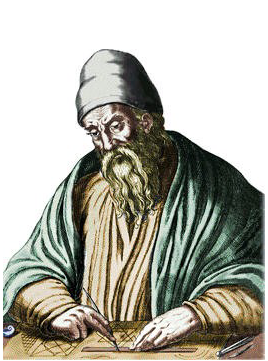
\includegraphics[width=1.0\linewidth]{./images/euklid.png}
  \captionof{figure}[Fantasieportrait Euklids. Das Bild wurde von Norbert Froese's Arbeit \textit{``Euklid und die Elemente. Die Entdeckung der axiomatischen Methode durch Euklid"} kopiert. Das ursprüngliche Bild stammt vom französischen Maler Charles Paul Landon (1760 – 1826). https://www.antike-griechische.de/Euklid.pdf. 2021)]{Euklid und die Elemente, 2021}
  \label{fig:portrait_euklid}
\end{minipage}
\vspace{.3cm}

``Um 300 v. Chr. veröffentlichte Euklid~\index{Euklid} die Bücher der
”Elemente“, die viele wichtige Erkenntnisse der
Primzahlforschung\index{Primzahl!Forschung}
mit korrekt geführten Beweisen beinhalteten'' (vgl. Sas
2002-2008, S. 4). Einer der wichtigen Beweise sind die
unendlich vielen Primzahlen.

\begin{theorem}[Satz von Euklid]
Es gibt unendlich viele Primzahlen.
\end{theorem}

\begin{proof}
(vgl. \cite{schichlsteinbauer}, S. 25).
\end{proof}

\newpage

%======================================================
\section{Primzahltests}
%======================================================

Wie im ersten Unterkapitel beschrieben, sind die Primzahlen
unendlich. Das heißt, dass es auch große Primzahlen
existieren, die für viele Verschlüsselungsverfahren immens
bedeutend sind.


%======================================================
% Chapter 2
%======================================================
%
% chap002.tex
%

\chapter{Kapitel 2}


%======================================================
% Chapter 3
%======================================================
%
% chap003.tex
%

\chapter{Die Summe der ersten $n$ ungeraden natürlichen Zahlen}

Mit Hilfe von farbigen Edelsteinen lassen sich quadratische Muster
auch auf andere Weise erzeugen. Ein quadratischer Haken, der
sogenannte \textit{Gnomon}, mit andersfarbigen Steinen wird
um ein vorhandene Steinquadrat aus $m \cdots m$ gelegt.
Dafür werden $m + 1 + m$, d.h. $2m + 1$, Steine benötigt.
Das entspricht einer ungerade Anzahl von Steinen.

Ein paare einfache Beispiele:
\[
 \begin{array}{l}
  1 + 3 = 4 = 2^2 \\ 
  1 + 3 + 5 = 9 = 3^2 \\ 
  1 + 3 + 5 + 7 = 16 = 4^2 \\ 
  1 + 3 + 5 + 7 + 9 = 25 = 5^2 \\
  \dots
 \end{array}
\]

\textbf{Regel: Summe der ersten n ungeraden Zahlen}

Die Folge der ersten $n$ ungeraden natürlichen Zahlen
kann als quadratisches Muster von Winkelhaken
dargestellt werden.

Die Summe der ersten $n$ ungeraden natürlichen Zahlen
ist gleich der Quadratzahl $n^2$.
\begin{equation}
  1 + 3 + 5 + \dots + (2n - 1) = n^2
  \label{eq:formel_ungerade_natuerliche_zahlen}
\end{equation}

\begin{proof}[\textbf{Beweis durch vollständige Induktion}]
 $\text{}$
 
 \begin{itemize}
  \item Induktionsanfang: $n = 1$
        \[
         \sum_{i=1}^{1} (2\cdot 1 - 1) = 1 = 1^2
        \]
  \item Induktionsvoraussetzung:\\  
        Es gelte
        \[
         \sum_{i=1}^{n} (2i - 1) = n^2
        \]
  \item Induktionsschritt: $n = n + 1$
        \[
         \begin{array}{rcl}
           \sum\limits_{i=1}^{n+1} (2i -1)
           & = & \sum\limits_{i=1}^{n} (2i -1) + 2(n+1)-1 \\\\
           & = & n^2 + 2n + 1 \\\\
           & = & (n+1)^2
         \end{array}
        \]
 \end{itemize}
\end{proof}

\begin{example}Summe der ungeraden natürlichen Zahlen von $1$ bis $9$.
 
 Zur Lösung dieses Beispiels kann man entweder die oben genannte
 Formel verwenden:
 \[
  \sum_{i=1}^{5} (2i -1) = 5^2 = 25
 \]

 Oder man kann auch mit der Figur rechnen:
 
 \begin{figure}[H]
  \centering
  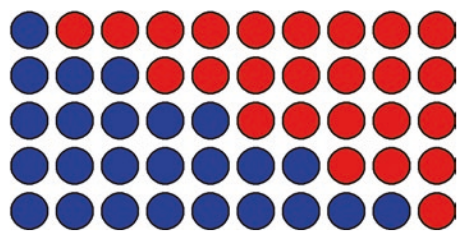
\includegraphics[width=.5\linewidth]{./images/muster03.png}
  \caption[]{Muster aus bunten Steinen zur Berechnung der Summe der ungeraden Zahlen $1,3,5,7,9$}
  \label{fig:muster_ungerade_1_bis_9}
\end{figure}

Zuerst legt man die blauen Steine in einer rechtwinkliger Dreicksform
von oben nach unten in aufsteigender Anzahl $1, 3, 5, 7, 9$ aus.
Danach verdoppelt man die Figur, indem man entsprechend viele rote Steine
von unten nach oben in absteigender Anzahl legt.
Als Resultat bekommt man eine Figure in Form eines Rechtecks.
Das Doppelte der Summe $1 + 3 + 5 + 7 + 9$ ist gleich $5\cdot 10 = 50$

Für die Summe $1 + 3 + 5 + 7 + 9$ ergibt sich der Wert $2\cdot 50 = 25$.
\end{example}
\vspace{.2cm}

\textbf{\textit{Aufgabe 2.5}:}
Begründen Sie: Eine weitere Möglichkeit der Herleitung der Formel
(\ref{eq:formel_ungerade_natuerliche_zahlen})
ergibt sich durch eine vielfache achsensymmetrische Anordnung von Steinen.

\begin{figure}[H]
  \centering
  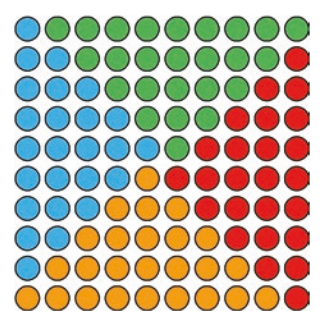
\includegraphics[width=.5\linewidth]{./images/muster04.png}
  \caption[]{}
  \label{fig:muster_ungerade_1_bis_9_achsensymmetrisch}
\end{figure}

\textbf{\textit{Lösung}:}
\[
  4 \cdot (1+3+5+7+9) = 8 \cdot (1+2+3+4+5) + 4\cdot 5
  = 8 \cdot \frac{1}{2}\cdot 4 \cdot 5 + 4 \cdot 5
  = 4 \cdot 4 \cdot 5 + 4 \cdot 5
  = 4^2 \cdot 5 + 4 \cdot 5
  = 4 \cdot 5^2
\]




%======================================================
% Chapter 4
%======================================================
%
% chap004.tex
%

\chapter{Quotienten von Summen ungerader natürlicher Zahlen}

Galileo Galilei (1564 - 1642) bemerkte, dass eine spezielle
Eigenschaft für gerade Anzahl aufeinanderfolgender ungerader
Zahlen erfüllt ist, nämlich:

\textit{
Das Verhältnis (Quotient) der Summe der ersten Hälfte der
ungeraden Zahlen zur Summe der verbleibenden
Hälfte der natürlichen Zahlen beträgt immer
$\frac{1}{3}$}.

\[
 \frac{1}{3} = \frac{1+3}{5+7} = \frac{1+3+5}{7+9+11}
 = \frac{1+3+5+7}{9+11+13+15} = \dots
\]

Aus diesem Quotienten erhält man die allgemeine Formel:
\[
 \frac{1}{3} = \frac{1+3+5+\dots+(2n-1)}{(2n+1)+(2n+3)+(2n+5)+\dots+(2n+(2n-1))}
\]



%======================================================
% Chapter 5
%======================================================
%
% chap005.tex
%

\chapter{Darstellung einer natürlichen Zahl als Summe aufeinanderfolgender
natürlicher Zahlen}

Es stehen zahlreiche Methoden zur Darstellung einer natürlichen Zahl
als Summe aufeinanderfolgender natürlicher Zahlen zur Verfügung.
Hier wird ein Beispiel zur Darstellung der Zahl $70$ als Summe
aufeinanderfolgender natürlicher Zahlen angeführt.

Um die Zahl $70$ darzustellen, hat man drei Möglichkeiten.
Die erste Möglichkeit ist die Aufteilung der Zahl $70$ in
zwei Mal $35$. Diese führt zu einen Rechteck mit 2 Reihen
mit jeweils 35 Steinen.

\begin{figure}[H]
  \centering
  
\includegraphics[width=.5\linewidth]{./images/muster05.png}
  \caption[]{Aufteilung der Zahl $70$ in zwei mal $35$.}
  \label{fig:muster_70_zweimal_35}
\end{figure}

$70$ ist eine gerade, durch 5 teilbare natürliche Zahl.
Man bildet $70$ durch $5 \cdot 14$.
Dadurch hat man ein Rechteck mit 5 Säulen, die jeweils
14 Steinen enthalten. Darüber hinaus gibt es eine
alternative Methode, bei der die Zahl $14$ um $1$ oder $2$
addiert oder subtrahiert wird, d.h.
$70 = 12 + 13 + 14 + 15 + 16$.
Also die Zahl $70$ lässt sich als Summe von 5 aufeinanderfolgenden
natürlichen Zahl darstellen.


%======================================================
% Chapter 6
%======================================================
%
% chap006.tex
%

\chapter{Summe der ersten $n$ Quadratzahlen von natürlichen Zahlen}

Abu Ali al-Hasan Ibn al-Haitham (965-1039), der im Deutschen unter
Alhazen und im Arabischen unter Ibn al-Haitham bekannt ist,
war ein bedeutender arabischer Mathematiker und Physiker.
Besondere wissenschaftliche Beiträge brachte er auf dem Gebiet
der Optik und der experimentellen Methodik.
Für seine Experimente auf diesem Gebiet gab man ihn den Beinamen
``Vater der Optik''. Es gilt als der Erfinder der Lupe und
damit der Mikroskopie. Die Formel zur Bestimmung der Summe der ersten
$n$ Quadratzahlen von natürlichen Zahlen wurde ebenfalls von
ihm entdeckt.

\begin{figure}[H]
  \centering
  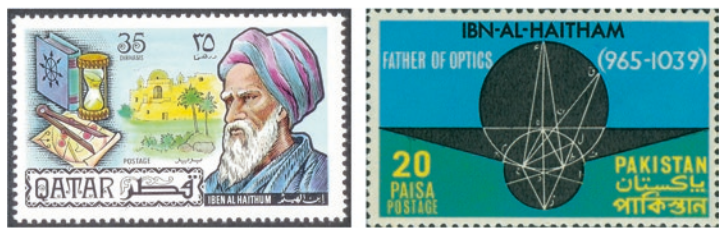
\includegraphics[width=.5\linewidth]{./images/muster06.png}
  \caption[]{Mathematiker und Physiker Abu Ali al-Hasan ibn al-Haitham (965-1039).}
  \label{fig:abu_ali_al_Hasan_ahitham}
\end{figure}




%======================================================
% Add appendix (Anhang)
%======================================================
\appendix{}

%======================================================
% Print the index list for later looking-up
%
% 1. Import package {makeindex}:
%       \usepackage{makeindex}
%
% 2. Add keyword "\makeindex" before/outside
%    "\begin{document}".
%
% 3. Add keyword "\printindex" within "\begin{document}".
%
% 4. Use keyword "\index{<entry>}" following a word
%    to add entry to index:
%       <Word>\index{<entry>}
%
% 5. Example:
%       \documentclass{article}
%       \usepackage[ngerman]{babel}
%       \usepackage{makeidx}
%       \makeindex
%
%       \begin{document}
%       ...
%           word1 word2 ... wordN\index{entry}
%       ...
%       \printindex
%       ...
%       \end{document}
%
%======================================================
\printindex

%======================================================
% Print the bibliography (Literatur)
%
% 1. Install Biber:
%       $ sudo apt install biber
%
% 2. Import package {biber} for creating bibliography:
%       \usepackage[backend=biber,style=numeric,]{biblatex}
%
% 3. Import package {csquotes} when working with "babel"
%    and "bibtex" to avoid the warning "'babel/polyglossia'
%    detected but 'csquotes' missing":
%
%       \usepackage[autostyle]{csquotes}
%
% 4. Add bibliography file before \begin{document}:
%       \addbibresource{bibliography.bib}
%
% 5. Add command for printing bibliography:
%       \printbibliography
%
% 6. Run in console:
%       $ pdflatex primzahlen.tex
%       $ biber primzahlen.bcf
%       $ pdflatex primzahlen.tex
%       $ pdflatex primzahlen.tex
%
%======================================================
\printbibliography

%======================================================
% Print list of figures (Abbildungsverzeichnis)
%
% 1. Import packages "\usepackage{graphicx}" and
%    "\usepackage{caption}".
% 2. Add "\listoffigures" within "\begin{doucment}".
% 3. Use "\begin{figure}"-environment and "\includegraphics"
%    to bind/display images.
% 4. Use "\caption[<short-title>]{<long-title>}" or
%    "\cationof{figure}[<list-entry-description>]{<title>}"
%    to assign caption to image and update image-list.
% 5. Compile .tex file twice:
%       $ pdflatex primzahlen.tex
%       $ pdflatex primzahlen.tex
%
%======================================================
\listoffigures

\backmatter{}% end of page numbering

\end{document}
